%versi 3 (22-07-2020)
\chapter{Analisis}
\label{chap:analisis}

Pada bab ini akan dijelaskan analisis aplikasi WSDC 2017 Bali saat ini dan aplikasi WSDC yang akan dibangun. Analisis yang akan dibahas meliputi analisis {\it use case}, analisis kebutuhan sistem, dan analisis pembangunan aplikasi Android menggunakan Ionic.

\section{Analisis Sistem Kini}
\label{sec:analisisSistemKini}
Aplikasi WSDC 2017 Bali digunakan untuk menunjang keberlangsungan acara WSDC 2017 yang diselenggarakan di Bali, Indonesia. Pada halaman utama, pengguna dapat melihat berita-berita terkait acara WSDC 2017 Bali dan tombol {\it read more} yang apabila ditekan akan mengarahkan pengguna untuk melihat berita terkait acara WSDC 2017 Bali dengan format pdf. Aplikasi WSDC 2017 Bali dapat digunakan untuk melihat berita acara, pengumuman, jadwal peserta, lokasi acara, hasil pengundian, info, serta pengumuman pemenang dari acara WSDC 2017 Bali (Gambar~\ref{fig:useCaseDiagram}). 

Aplikasi WSDC 2017 Bali dibangun menggunakan {\it framework} Ionic versi 3, dan Angular versi 4.1.3. Dengan digunakannya Ionic Framework, maka memungkinkan aplikasi WSDC 2017 Bali menggunakan teknologi web seperti HTML, dan CSS. Lalu untuk membangun aplikasi WSDC 2017 Bali agar dapat berjalan secara {\it native}, digunakanlah Cordova. Penggunaan Cordova memungkinkan aplikasi WSDC 2017 Bali kompatibel dengan perangkat berbasis Android dan IOS, tanpa perlu mengimplementasikannya kembali ke dalam bahasa masing-masing platform.

\begin{figure}[H]
		\centering
	    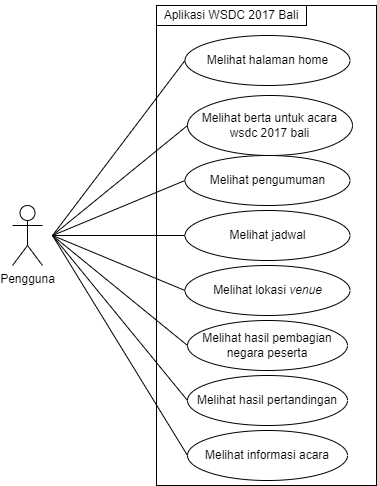
\includegraphics[scale=0.4]{Gambar/useCaseDiagram.png}
	    \caption{{\it Use Case Diagram} Aplikasi WSDC 2017 Bali}
	    \label{fig:useCaseDiagram}
\end{figure}

Terdapat {\it sidebar} untuk pengguna agar dapat bernavigasi ke dalam menu-menu yang terdapat pada aplikasi WSDC 2017 Bali. Untuk mengakses {\it sidebar}, pengguna dapat menekan tombol navigasi berada di sebelah kiri atas aplikasi WSDC 2017 Bali. Selain itu dapat pula dengan cara mengusap layar dari kiri ke kanan. Untuk menutup {\it sidebar}, pengguna dapat menekan area di luar {\it sidebar}, atau dengan cara menekan tombol silang di sebelah kiri atas {\it sidebar}. Terdapat fitur-fitur yang ada pada aplikasi WSDC 2017 Bali yang dapat diakses melalui {\it sidebar}. Fitur-fitur tersebut adalah sebagai berikut :
\begin{enumerate}
	\item Halaman Utama : Pengguna dapat melihat halaman utama aplikasi WSDC 2017 Bali yang berisi berita acara WSDC 2017 Bali, serta pemberitahuan terakhir terkait acara WSDC 2017 Bali.
	\begin{itemize}
		\item Nama: Melihat Halaman Utama WSDC 2017 Bali.
		\item Aktor: Pengguna Aplikasi WSDC 2017 Bali.
		\item Deskripsi: Pengguna melihat halaman awal yang berisi berita acara WSDC 2017 Bali dengan urutan paling atas adalah berita yang lebih baru terbit, dan sebuah {\it card} yang berisi pengumuman terakhir terkait acara WSDC 2017 Bal, yang dapat diklik dan mengarahkan pengguna ke halaman Pemberitahuan.
		\item Kondisi Awal: Pengguna belum membuka aplikasi WSDC 2017 Bali.
		\item Kondisi Akhir: Aplikasi menampilkan halaman utama aplikasi WSDC 2017 Bali.
		\item Skenario utama:\\
		\begin{table}[H]
			\centering
			\begin{tabular}{|p{0.5cm}|p{7cm}|p{7cm}|}
				\hline
				No & Aksi Aktor                               & Reaksi Sistem                                          \\ \hline
				1  & Pengguna membuka aplikasi WSDC 2017 Bali & Aplikasi WSDC 2017 Bali menampilkan halaman selamat datang. \\ \hline
				2  &                                          & Aplikasi WSDC 2017 Bali menampilkan halaman utama           \\ \hline
				3  & Pengguna mengklik {\it card} Announcements & Aplikasi WSDC 2017 Bali menampilkan halaman Pemberitahuan. \\ \hline
			\end{tabular}
			\caption{Tabel Skenario dari Halaman Utama}
			\label{table:skenarioHalamanUtama}
		\end{table}
	\end{itemize}
	\item Berita : Pengguna dapat melihat berita acara WSDC 2017 Bali dengan format pdf.
	\begin{itemize}
		\item Nama: Melihat Berita Acara WSDC 2017 Bali.
		\item Aktor: Pengguna aplikasi WSDC 2017 Bali.
		\item Deskripsi: Melihat berita acara dengan format pdf yang berisi kejadian kejadian pada WSDC 2017 Bali di tanggal tertentu sesuai dengan berita yang diklik.
		\item Kondisi Awal: Pengguna telah membuka halaman utama aplikasi WSDC 2017 Bali.
		\item Kondisi Akhir : Berkas berita WSDC 2017 Bali dengan format pdf dapat dilihat dan dibaca.
		\item Skenario Utama: \\
		\begin{table}[H]
			\centering
			\begin{tabular}{|p{0.5cm}|p{7cm}|p{7cm}|}
				\hline
				No & Aksi Aktor                               & Reaksi Sistem                                          \\ \hline
				1  & Pengguna menekan tombol {\it read more} pada berita di halaman utama aplikasi WSDC 2017 Bali. & Aplikasi WSDC 2017 Bali mengarahkan pengguna ke halaman Google Drive yang menampilkan berita acara WSDC 2017 Bali \\ \hline
				2  &  & Aplikasi WSDC 2017 Bali menampilkan berita acara WSDC 2017 Bali \\ \hline
			\end{tabular}
			\caption{Tabel Skenario dari Berita}
			\label{table:skenarioBerita}
		\end{table}
	\end{itemize}
	\item Pengumuman : Pengguna dapat melihat pengumuman mengenai keberlangsungan acara WSDC 2017 Bali.
	\begin{itemize}
		\item Nama: Melihat pemberitahuan acara WSDC 2017 Bali.
		\item Aktor: Pengguna aplikasi WSDC 2017 Bali.
		\item Deskripsi: Melihat pemberitahuan acara WSDC 2017 Bali yang tersusun menurun berdasarkan jam dan tanggal dirilisnya pengumuman tersebut.
		\item Kondisi Awal: Pengguna telah membuka aplikasi WSDC 2017 Bali.
		\item Kondisi Akhir: Halaman pemberitahuan terbuka dan menampilkan pemberitahuan acara WSDC 2017 bali yang tersusun menurun berdasarkan jam dan tanggal.
		\item Skenario utama: \\
		\begin{table}[H]
			\centering
			\begin{tabular}{|p{0.5cm}|p{7cm}|p{7cm}|}
				\hline
				No & Aksi Aktor                               & Reaksi Sistem                                          \\ \hline
				1  & Pengguna menekan tombol {\it hamburger} di pojok kiri atas aplikasi WSDC 2017 Bali. & Aplikasi WSDC 2017 Bali menampilkan {\it sidebar} \\ \hline
				2  & Pengguna menekan tombol Announcement & Aplikasi WSDC 2017 Bali menampilkan halaman pengumuman. \\ \hline
			\end{tabular}
			\caption{Tabel Skenario dari Halaman Pemberitahuan}
			\label{table:skenarioHalamanPemberitahuan}
		\end{table}
	\end{itemize}
	\item Jadwal : Pengguna dapat melihat jadwal acara WSDC 2017 Bali yang ditampilkan berdasarkan tanggal dan hari.
	\begin{itemize}
		\item Nama: Melihat jadwal acara WSDC 2017 Bali.
		\item Aktor: Pengguna aplikasi WSDC 2017 Bali.
		\item Deskripsi: Melihat jadwal acara WSDC 2017 Bali yang ditampilkan berdasarkan tanggal dan hari, serta dapat berpindah pindah tanggal agar dapat melihat jadwal apa saja yang tersedia pada hari itu. Untuk setiap harinya terdapat nama kegiatan, waktu yang menunjukan pukul berapa acara tersebut mulai dan selesai, serta lokasi kegiatan acara tersebut.
		\item Kondisi awal: Pengguna telah membuka aplikasi WSDC 2017 Bali.
		\item Kondisi akhir: Halaman jadwal terbuka dan menampilkan jadwal acara yang ditampilkan berdasarkan tanggal dan hari, serta dapat melihat acara dengan detail waktu, tempat, dan nama kegiatan.
		\item Skenario utama: \\
		\begin{table}[H]
			\centering
			\begin{tabular}{|p{0.5cm}|p{7cm}|p{7cm}|}
				\hline
				No & Aksi Aktor                               & Reaksi Sistem                                          \\ \hline
				1  & Pengguna menekan tombol {\it hamburger} di pojok kiri atas aplikasi WSDC 2017 Bali. & Aplikasi WSDC 2017 Bali menampilkan {\it side bar} \\ \hline
				2  & Pengguna menekan tombol Schedule & Aplikasi WSDC 2017 Bali menampilkan halaman jadwal. \\ \hline
				3  & Pengguna menekan tanggal yang berada di atas halaman jadwal & Aplikasi WSDC 2017 Bali menampilkan jadwal berdasarkan tanggal yang dipilih oleh pengguna dengan detail waktu, lokasi, dan nama kegiatan. \\ \hline
			\end{tabular}
			\caption{Tabel Skenario dari Halaman Jadwal}
			\label{table:skenarioHalamanJadwal}
		\end{table}
	\end{itemize}
	\item {\it Venues} : Pengguna dapat melihat lokasi dari berlangsungnya acara WSDC 2017 Bali.
	\begin{itemize}
		\item Nama: Melihat lokasi acara WSDC 2017 Bali.
		\item Aktor: Pengguna aplikasi WSDC 2017 Bali.
		\item Deskripsi: Pengguna dapat melihat lokasi dari berlangsungnya acara WSDC 2017 Bali, yang dibagi menjadi 4 kategroi, yaitu: {\it Ceremony Venues}, {\it Competition Venues}, {\it Delegates Accomodation}, dan {\it Educational Tour}. Masing masing dari lokasi tersebut akan menampikan peta, dan lokasi acara yang dituju dengan penanda yang ada di dalam peta. Serta dapat menampilkan jarak pengguna saat ini terhadap lokasi yang ingin dituju.
		\item Kondisi awal: Pengguna telah membuka aplikasi WSDC 2017 Bali.
		\item Kondisi akhir: Halaman {\it venues} yang sesuai dengan keinginan pengguna terbuka.
		\item Pengecualian: Aplikasi WSDC 2017 Bali tidak akan menampilkan jarak antara lokasi pengguna saat ini ke lokasi yang ingin dituju, jika pengguna berada di luar pulau Bali.
		\item Skenario utama: \\
		 \begin{table}[H]
			\centering
			\begin{tabular}{|p{0.5cm}|p{7cm}|p{7cm}|}
				\hline
				No & Aksi Aktor                               & Reaksi Sistem                                          \\ \hline
				1  & Pengguna menekan tombol {\it hamburger} di pojok kiri atas aplikasi WSDC 2017 Bali. & Aplikasi WSDC 2017 Bali menampilkan {\it sidebar} \\ \hline
				2  & Pengguna menekan tombol Venues & Aplikasi WSDC 2017 Bali menampilkan halaman Venues yang berisi {\it Ceremony Venues}, {\it Competition Venues}, {\it Delegates Accomodation}, dan {\it Educational Tour}.\\ \hline
				3  & Pengguna menekan kategori {\it venues} yang diinginkan. & Aplikasi WSDC 2017 Bali menampilkan peta, nama lokasi acara dengan disertai penanda yang ada di dalam peta, dan jarak antara lokasi pengguna saat ini dan lokasi acara.\\ \hline
			\end{tabular}
			\caption{Tabel Skenario dari Halaman {\it Venues}}
			\label{table:skenarioHalamanVenues}
		\end{table}
	\end{itemize}
\newpage
	\item {\it Draw} : Pengguna dapat melihat pembagian {\it venue} serta pembagian kubu proposisi dan oposisi dari hasil pengundian untuk para negara peserta WSDC 2017 Bali.
	\begin{itemize}
		\item Nama: Melihat halaman {\it draw}
		\item Aktor: Pengguna aplikasi WSDC 2017 Bali.
		\item Deskripsi: Pengguna dapat melihat hasil dari pengundian kubu untuk negara peserta WSDC 2017 Bali, yaitu kubu proposisi dan oposisi, serta lokasi {\it venue} untuk kedua kubu tersebut. Aplikasi WSDC 2017 Bali akan menampilkan nama-nama negara peserta dengan benderanya masing-masing yang terbagi menjadi dua kubu di dalam satu tabel, kubu oposisi dan kubu proposisi.
		\item Kondisi awal: Pengguna telah membuka aplikasi WSDC 2017 Bali.
		\item Kondisi akhir: Halaman {\it draw} terbuka.
		\item Skenario utama: \\
		\begin{table}[H]
			\centering
			\begin{tabular}{|p{0.5cm}|p{7cm}|p{7cm}|}
				\hline
				No & Aksi Aktor                               & Reaksi Sistem                                          \\ \hline
				1  & Pengguna menekan tombol {\it hamburger} di pojok kiri atas aplikasi WSDC 2017 Bali. & Aplikasi WSDC 2017 Bali menampilkan {\it side bar} \\ \hline
				2  & Pengguna menekan tombol Draw & Aplikasi WSDC 2017 Bali menampilkan halaman Draw yang dapat digulir kebawah untuk menampilkan keseluruhan tabel. \\ \hline
			\end{tabular}
			\caption{Tabel Skenario dari Halaman {\it Draw}}
			\label{table:skenarioHalamanDraw}
		\end{table}
	\end{itemize}
	\item Hasil : Pengguna dapat melihat pemenang dari kompetisi WSDC 2017 Bali.
	\begin{itemize}
		\item Nama : Melihat halaman Hasil.
		\item Aktor: Pengguna aplikasi WSDC 2017 Bali.
		\item Deskripsi: Pengguna dapat melihat pemenang dari kompetisi WSDC 2017 Bali, yang terdiri dari babak semifinal, perempatfinal, dan perdelapanfinal. Dari masing-masing babak, ditampilkan negara-negara yang berpartisipasi, serta skor dari negara-negara tersebut. 
		\item Kondisi awal: Pengguna telah membuka aplikasi WSDC 2017 Bali.
		\item Kondisi akhir: Halaman Hasil terbuka.
		\item Skenario utama: \\
		\begin{table}[H]
			\centering
			\begin{tabular}{|p{0.5cm}|p{7cm}|p{7cm}|}
				\hline
				No & Aksi Aktor                               & Reaksi Sistem                                          \\ \hline
				1  & Pengguna menekan tombol {\it hamburger} di pojok kiri atas aplikasi WSDC 2017 Bali. & Aplikasi WSDC 2017 Bali menampilkan {\it side bar} \\ \hline
				2  & Pengguna menekan tombol Result & Aplikasi WSDC 2017 Bali menampilkan halaman Result yang berisi pemenang dari babak semifinal, perempatfinal, dan perdelapanfinal. \\ \hline
			\end{tabular}
			\caption{Tabel Skenario dari Halaman Hasil}
			\label{table:skenarioHalamanHasil}
		\end{table}
	\end{itemize}
\newpage
	\item Info : Pengguna dapat melihat info-info seputar kontak-kontak penting yang dapat dihubungi, kosa kata dalam Bahasa Indonesia sehari-hari, serta {\it credits} kepada pembuat aplikasi WSDC 2017 Bali.
	\begin{itemize}
		\item Nama: Melihat halaman Info.
		\item Aktor: Pengguna aplikasi WSDC 2017 Bali.
		\item Deskripsi: Pengguna dapat melihat info kontak-kontak yang dapat dihubungi, dengan menekan nomor telepon yang ada di halaman Info. Setelah menekan nomor telepon tersebut, pengguna akan diarahkan ke aplikasi pemanggilan. Lalu ada juga informasi mengenai kosa kata dalam Bahasa Indonesia, yang dapat dipakai oleh pengguna, khususnya peserta WSDC 2017 Bali dari mancanegara. Serta terdapat pula informasi mengenai siapa saja yang berperan dalam pembuatan aplikasi WSDC 2017 Bali.
		\item Kondisi awal: Pengguna telah membuka aplikasi WSDC 2017 Bali.
		\item Kondisi akhir: Halaman Info terbuka.
		\item Skenario utama: \\
		\begin{table}[H]
			\centering
			\begin{tabular}{|p{0.5cm}|p{7cm}|p{7cm}|}
				\hline
				No & Aksi Aktor                               & Reaksi Sistem                                          \\ \hline
				1  & Pengguna menekan tombol {\it hamburger} di pojok kiri atas aplikasi WSDC 2017 Bali. & Aplikasi WSDC 2017 Bali menampilkan {\it side bar} \\ \hline
				2  & Pengguna menekan tombol Info & Aplikasi WSDC 2017 Bali menampilkan halaman Info \\ \hline
			\end{tabular}
			\caption{Tabel Skenario dari Halaman Info}
			\label{table:skenarioHalamanInfo}
		\end{table}
	\end{itemize}
\end{enumerate}

\section{Analisis Sistem Usulan}
\label{sec:analisisSistemUsulan}

Aplikasi yang ada pada saat ini menggunakan Ionic Framework versi 3, yang sudah tidak lagi didukung oleh Ionic. Maka dari itu, aplikasi WSDC 2017 Bali akan dibangun ulang  menggunakan Ionic Framework versi terbaru saat ini, yaitu Ionic Framework versi 5. Proses untuk melakukan pembangunan ulang aplikasi dari Ionic Framework versi 3 ke Ionic Framework versi 5 telah dijelaskan pada sub bab~\ref{subsec:migrasi}. Pada sub bab ini akan dijelaskan analisis untuk pengembangan kebutuhan apilkasi WSDC 2017 Bali agar aplikasi tersebut dapat berjalan menggunakan Ionic Framework versi 5.

\subsection{Analisis Kebutuhan Sistem Usulan}
\label{sec:analisisKebutuhanSistem}
Aplikasi WSDC 2017 Bali yang akan dibangun akan mengadopsi desain dan tata letak yang sama persis dengan aplikasi WSDC 2017 Bali saat ini. Namun dengan perubahan penggunaan Ionic Framework yang digunakan, yaitu versi 5, serta Angular versi 12. Di Ionic Framework terbaru saat ini, aplikasi WSDC 2017 Bali yang akan dibangun akan memanfaatkan fasilitas yang disediakan oleh Ionic Framework, yaitu UI Component, dan CSS Utilities. 

Bagian-bagian dari UI Component yang akan digunakan pada aplikasi WSDC 2017 Bali yang akan dibangun diantaranya yaitu :
\newpage
\begin{itemize}
	\item Button \\
	Komponen ini akan digunakan untuk membuat suatu elemen yang dapat diklik. Contoh dari penggunaan Button adalah pada halaman Berita, yang penggunaannya dapat dilihat pada sub bab~\ref{sec:analisisSistemKini} bagian Berita, yaitu untuk mengklik tombol {\it read more} dan mengarahkan pengguna ke aplikasi penampil pdf.
	\item Card \\
	Komponen ini akan digunakan sebagai tampilan antar muka, yang dapat menjadi titik masuk ke dalam informasi yang lebih detail. Contoh dari pneggunaan Card adalah pada halaman utama, yaitu pengguna dapat menekan Card Announcements, dan akan diarahkan ke halaman Pengumuman. Contoh dari penggunaan Card pada halaman utama dapat dilihat pada sub bab~\ref{sec:analisisSistemKini}.
	\item Content \\
	Komponen ini akan digunakan sebagai penyedia area konten yang digunakan untuk mengontrol area yang dapat digulir. Penggunaan Content ada pada setiap halaman, agar halaman tersebut dapat digulir dan menampilkan isi konten dari halaman tersebut.
	\item Icon \\
	Komponen ini akan digunakan untuk merepresentasikan sebuah halaman yang ada pada side-menu.
	\item Item \\
	Komponen ini akan digunakan sebagai pembungkus dari komponen-komponen lain di dalam sebuah halaman. Item akan berisi teks, gambar, atau elemen lainnya.
	\item Menu \\
	Komponen ini akan digunakan sebagai tempat bagi pengguna untuk mengakses berbagai halaman yang tersedia. Pada aplikasi WSDC 2017 Bali saat ini, terdapat sebuah menu berjenis \textit{side bar}, yang berisi tombol untuk bernavigasi ke halaman-halaman yang ada. 
	\item Segment \\
	Komponen ini akan digunakan untuk pengguna agar dapat berpindah tampilan di dalam halaman yang sama. Seperti pada tampilan halaman jadwal yang ada pada aplikasi WSDC 2017 Bali saat ini, dimana pengguna dapat berpindah hari untuk mengetahui jadwal kegiatan pada hari tertentu yang dipilih oleh pengguna, namun masih berada di halaman yang sama, yaitu halaman Schedule.
	\item Toolbar \\
	Komponen ini akan digunakan sebagai header dari aplikasi WSDC 2017 Bali. Dalam Toolbar, akan terdapat tombol navigasi yang dapat diklik untuk menampilkan side-menu yang dapat digunakan pengguna untuk bernavigasi antar halaman. Lalu terdapat pula tulisan nama halaman yang saat ini sedang dibuka oleh pengguna, serta logo WSDC 2017 Bali.
\end{itemize}

Lalu, aplikasi WSDC 2017 Bali yang akan dibangun juga akan memanfaatkan CSS Utilities yang disediakan oleh Ionic Framework. CSS Utilities milik Ionic Framework menyediakan satu set kelas CSS yang akan digunakan pada elemen-elemen di dalam aplikasi, untuk memodifikasi teks, penempatan elemen, atau penyesuaian dari padding dan margin.

\subsection{Permasalahan Pengembangan Sistem Usulan}
\label{sec:analisisPermasalahanSistemKini}
Saat sedang melakukan proses migrasi aplikasi WSDC 2017 Bali dari Ionic Framework versi 3 ke Ionic Framework versi 5, terdapat beberapa kendala yang dialami. Kendala-kendala tersebut adalah sebagai berikut : 
\begin{itemize}
	\item Seperti yang disebutkan pada landasan teori (Sub Bab~\ref{subsec:migrasi}) sebelum melakukan migrasi dari Ionic Framework versi 3 ke Ionic Framework versi 5 terlebih dahulu melakukan migrasi dari Ionic Framework versi 3 ke Ionic Framework versi 4. Namun karena tidak tersedianya perintah untuk membuat aplikasi dengan menggunakan Ionic Framework versi 4, maka penulis langsung melakukan migrasi dari Ionic Framework versi 3 ke Ionic Framework versi 5. Dalam melakukan hal ini, penulis berlandaskan bahwa susunan kelas Ionic Framework versi 4 dan versi 5 tidaklah berubah sama sekali. Yang mengalami perubahan hanyalah pembaruan properti mengenai API, CSS, dan {\it package dependencies} yang terpasang, yang telah dijelaskan pada landasan teori (Sub Bab~\ref{subsec:migrasi}).
	\item Halaman Draw dan Result pada aplikasi WSDC 2017 Bali saat ini tidak dapat diakses dikarenakan data pada server yang tersedia tidak dapat diakses. Namun masalah ini telah terselesaikan.
\end{itemize}
%Analisis cara kerja ionicnya
%Analisis cara kerja cordova
%Analisis isi dari aplikasinya bakal pake apa aja, contoh bakal ada maps, sama lokasi
%Jelasin gimana bisa jadi aplikasi wsdcnya, pake apa biar bisa jadi apk nya
